\chapter{Continuous function on metric spaces}
\section{Continuous functions}
\paragraph{Excercise 2.1.1}
\begin{itemize}
\item[(a)$\Rightarrow$(b)]Let $(x^{(n)})_{n=1}^{\infty}$ a sequence converges to $x_{0}$. For fucntion $f$ is continuous, $\forall \varepsilon$ $\exists \delta$ s.t. when $d(x_{0},x)<\delta$, $d(f(x),f(x_{0}))<\varepsilon$. For $(x^{(n)})_{n=1}^{\infty}$ converges to $x_{0}$, there exists $N$ when $n>N$, $d(x^{(n)},x_{0})<\delta$. Therefore, $d(f(x^{(n)}),f(x_{0}))<\varepsilon$ when $n>N$.
\item[(b)$\Rightarrow$(c)] Prove its conter proposition. Assume for every open set $V \subset Y$ that contains $f(x_{0})$, for any open sets $U \subset X$ containing $x_{0}$, $f(U)\nsubseteq V$ which means there exists a point $x^\prime\in U$; $f(x^\prime)\notin V$. From above, we know we can construct a sequence $a_{n}\rightarrow x_{0}$ whose $(f(x^{(n)}))_{n=1}^{\infty}$ doesn't converges to $f(x_{0})$ \Lightning. Therefore, statement does hold.
\item[(c)$\Rightarrow$(a)]
Patently.
\end{itemize}
\paragraph{Excercise 2.1.2}
\begin{itemize}
\item[(a)$\Rightarrow$(c)] Form previous excercise, we know that\\ {\it For every open set $V \subset Y$ that contains $f(x_{0})$, there exists an open set $U \subset X$ containing $x_{0}$ such that $f(U) \subset V$.}\dots(1)
\\
For a point $x^\prime$ in $f^{-1}(V)$, $f(x^\prime)$ belongs to $V$ which is open. There exists a open set $B_{r}(f(x^\prime))$ in $V$. By (1), there exists a open set $U^\prime \subset X$ containing $x^\prime$ such that $f(U^\prime) \subseteq V$. The existance of $U^\prime$ implies $f^{-1}(V)$ is open.
\item[(c)$\Rightarrow$(a)] Similiarly, prove (c) can $\Rightarrow$ (1).
\item[(c)$\Rightarrow$(d)]With proposition 1.2.5.(e), and proposition 1.3.4, it is easy to see. 
\end{itemize}
\paragraph{Excercise2.1.6}
The right direction is induced. However, the reverse direction is wrong.For example, the dilichlet function is continuous in $\mathbb{Q}$, but not in $\mathbb{R}$.
\section{Continuity and product spaces}
\paragraph{Excercise2.2.5}
\begin{proof}
From excercise 2.2.4, we know that $P_{1}(x,y)=x$ is a continuous function. By corollary 2.2.3, we know that $P_{2}(x,y)=c_{ij}x\times y$ is also continuous. By induction, we know that $P(x,y)=\sum_{i=0}^{n}\sum_{j=0}^{m}c_{if}x^{i}y^{j}$ is continuous.
\end{proof}
\paragraph{Excercise2.2.7} We have already
find that, when $k=2$, statement holds. Assume it holds for $k=n$ (\[P(x_{1},\dots,x_{n}):=\sum_{(i_{1},\dots,i_{n})\in I}c(i_{1},\dots,i_{n})x_{1}^{i_{1}}\dots x_{n}^{i_{n}}\qquad\dots(1)\] is continuous) , let's show it is also true for $k=n+1$.\\ Patently, each term of $P(x_{1},\dots,x_{n+1})$ is continuous.\dots (2) (why is that, see following)\\
Because, from (1), for any particular $(i_{1},\dots,i_{n},i_{n+1})\in I$, function $y=c(i_{1},\dots,i_{n},i_{n+1})x_{1}^{i_{1}}\dots x_{n}^{i_{n}}$ is continuous. In addition, function $y=x_{n+1}^{i_{n+1}}$ is continuous. Therefore, (2) holds with the help of limit law. For $I$ is finite, we can use corollary 2.2.3 (b) finitely many times to finish the proof.
\paragraph{Excercise2.2.8\textcolor{red}{Toberemained}} In fact, this isn't quite clear to me. However, I will have a try. The following is the analogue of proposition 1.1.18.\\
Let $X\times Y$ be the metric space that mentioned in the book, let $(x^{(k)})_{k=m}^{\infty}$ be a sequence of points in $X\times Y$. We write $x^{(k)}
=((x_{1}^{(k)},x_{2}^{(k)},\dots,x_{m}^{(k)}),(x_{1}^{(k)},x_{2}^{(k)},\dots,x_{n}^{(k)}))$, i.e., for \\
\dots, I am tired. I don't want to think it out explicitly and type it down.

\paragraph{Excercise 2.2.9}
I will only show $\lim_{x\rightarrow x_{0}}\limsup_{y\rightarrow y_{0}}f(x,y)=f(x_{0},y_{0})$
\begin{figure}[H]
\centering
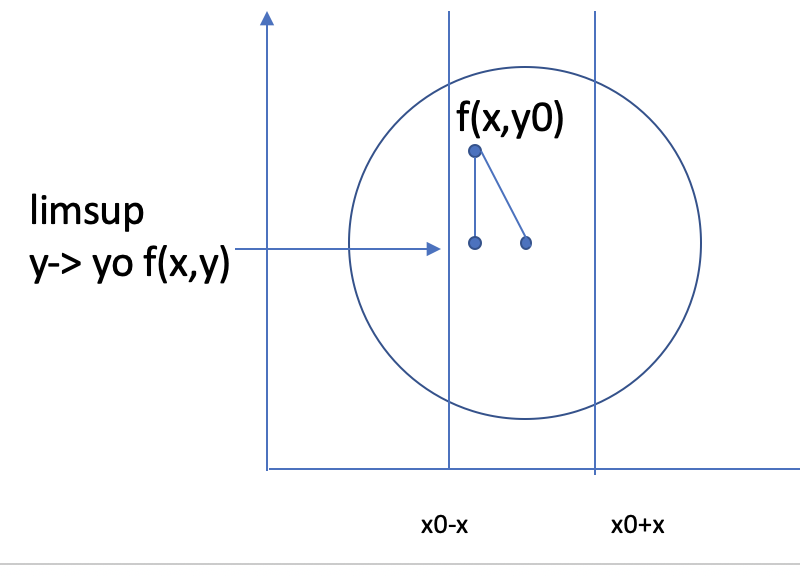
\includegraphics[width=8cm]{Excercise229}
\caption{Intuition figure}
\end{figure}
\begin{proof}
$\forall\varepsilon$ $\exists \delta$ s.t. for all $d((x,y),(x_{0},y_{0}))<\delta$, $|f(x,y)-f(x_{0},y_{0})|<\varepsilon$.\\Then for $|x^\prime-x_{0}|<\frac{\sqrt{2}\delta}{2}$, there exists $|y^\prime-y_{0}|<\frac{\sqrt{2}\delta}{2}$;
\[|f(x^\prime,y^\prime)-\limsup_{y\rightarrow y_{0}}f(x^\prime,y)|<\varepsilon\]
In addition, for $d((x^\prime,y^\prime),(x_{0},y_{0}))<\delta$,
\[|f(x^\prime,y^\prime)-f(x_{0},y_{0})|<\varepsilon
\]
Therefore,
\[|f(x_{0},y_{0})-\limsup_{y\rightarrow y_{0}}f(x^\prime,y)|<2\varepsilon
\]


\end{proof}
\section{Continuity and compactness}
\paragraph{Excercise2.3.1}
For any sequence $\{f(x_{n})\}_{n}$ in $f(K)$, there exists a convergent subsequence $\{x_{n^\prime}\}_{n^\prime}$. Then the subsequence $\{f(x_{n^\prime})\}_{n^\prime}$ of $\{f(x_{n})\}_{n}$ is convergent because of continuity of $f$.
\paragraph{Excercise2.3.2}First, want to show that: $f$ is bounded. Assuem $f$ isn't bounded, then we can construct a sequence $\{x_{n}\}_{n}$ such that it goes to infinity. Because of the compactness of $X$, there exists a convergent subsequence $\{x_{n^\prime}\}_{n^\prime}$ whose image
$\{f(x_{n^\prime})\}_{n^\prime}$ diverges. This contradict to the fact that $f$ is continuous.\\
Secondly, set the $sup(f(X))$ be a. If there exists a $x$ that $f(x)=a$, then we are done. If not, we can  which means we can construct a monotone increasing sequence $\{f(x_{n})\}_{n}\rightarrow a$. Again, for $X$ is compact, there exists a convergent subsequence $\{x_{n^\prime}\}_{n^\prime}\rightarrow x_{0}$ of $\{x_{n}\}_{n}$. $f(x_{0})=a$ because of continuity of $f$  \Lightning.
\section{Continuity and connectedness}
\paragraph{Excercise 2.4.1} For a element $x$ in $E$, then $E=\{x\}\cup (E/\{x\})$. In particular,$\{x\}$ and $(E/\{x\})$ are open set( for any point, consider those neighbourhood with radius less than $\frac{1}{2}$).
\paragraph{Excercise 2.4.3} I don't know how to show $(b)\rightarrow(c)$.
\paragraph{Excercise 2.4.6} 
\begin{proof}
Assume $f(E)$ is not connected; $f(E)=U\cup V$, where $U$ and $V$ are disjoint. For $f$ is continuous, $f^{-1}(U)$ and $f^{-1}(V)$ are open set. Then $f^{-1}(U)\cap f^{-1}(V)\neq\emptyset$ because of connectedness of $E$. For a point $x\in f^{-1}(U)\cap f^{-1}(V)$, we can see that $f(x)\in U$ and $f(x)\in V$ which is ridiculous. Therefore, $f(E)$ is connected.
\paragraph{Excercise2.4.6}For any two open set, $V$ and $W$, satisfied $U\cup W=\bigcup_{\alpha\in I}E_{\alpha}$, we want to show they are adjoint. 
\[
\bigcup_{\alpha\in I}E_{\alpha}=\{\bigcap_{\alpha\in I}E_{\alpha}\}\cup\{\bigcup_{\alpha\in I}E_{\alpha}/\bigcap_{\alpha\in I}E_{\alpha}\}
\]
w.l.o.g. assume an element $a\in\bigcap_{\alpha\in I}E_{\alpha}$ is in $W$. Then, for $V$ is non-empty, there is a element $b\in E_{\alpha^\prime}$ for $\alpha^\prime\in I$. From above, we can draw the conclusion that:$W\cap E_{\alpha^\prime}\neq\emptyset$ and $V\cap E_{\alpha^\prime}\neq\emptyset$.\\ In addition, $\{V\cap E_{\alpha^\prime}\}\cup\{W\cap E_{\alpha^\prime}\}=\{V\cup W\}\cap E_{\alpha^\prime}=\bigcup_{\alpha\in I}E_{\alpha}\cap E_{\alpha^\prime}=E_{\alpha^\prime}$\dots (1). Now, we know (1), $\{V\cap E_{\alpha^\prime}\}$ is open w.r.t. $(E_{\alpha^\prime},d_{E_{\alpha^\prime}\times E_{\alpha^\prime}})$ (so does $W$) and $E_{\alpha^\prime}$ is connected. Then $\{V\cap E_{\alpha^\prime}\}\cap\{W\cap E_{\alpha^\prime}\}\neq\emptyset$, so is $V\cap W$.
\end{proof}
\paragraph{Excercise2.4.7}For two non-empty open sets $V$, $W$ satisfied $V\cup W=E$, we pick $a\in V$ and $b\in W$. There is a conituious function $\gamma:[0,1]\rightarrow E$ such that $\gamma(0)=a,\gamma(1)=b$. Then $\gamma([0,1])$ is connected. Union of two open sets $(V\cap\gamma([0,1])) \cup (W\cap\gamma([0,1]))$ equal $\gamma([0,1])$ $(V\cap\gamma([0,1])) \cap (W\cap\gamma([0,1]))\neq\emptyset$.
Therefore, $V\cap W\neq\emptyset$. 
\paragraph{\textcolor{red}{Excercise2.4.9}} I havn't solve this question. Never mind, I'll just keep going.
\section{Topological spaces (Optional)}
\paragraph{Excercise 2.5.4}Assume $\{x^{(n)}\}_{n}$ converges to x. Then W.T.S that for any $a\neq x$, $\{x^{(n)}\}_{n}$ doesn't converge to $a$ for Hausdorff topological space. There exist two sets $U$, $W$ s.t. $x\in U$, $y\in W$ and $U\cap W=\emptyset$. Then there exists an $N$ s.t. for $n>N$, $x^{(n)}\in U$. Which means there exists a neighbourhood $W$ of $a$ such that there doesn't exist an $N$ such that $x^{(n)}\in W$ for all $n>N$.\\
Counter-example:$(X,\mathcal{F})$,$X={a,b,c}$, $\mathcal{F}=\{\{a,b,c\}\{a,b\}\{c\}\}$. Then, $a,\dots, a,\dots$ converges both a and b.
\paragraph{\textcolor{red}{Excercise 2.5.6}}

















